% Chapter 4: Artificial Intelligence Features
\chapter{Artificial Intelligence Features}

\chapterquote{Artificial intelligence is the new electricity.}{Andrew Ng}

\section*{Introduction}
\addcontentsline{toc}{section}{Introduction}

This chapter explores the integration of artificial intelligence capabilities within our real estate platform. We have developed four distinct AI models, each addressing specific needs within the ecosystem. These models collectively enhance user experience, improve decision-making processes, and provide valuable insights to various stakeholders in the real estate market.

The AI features presented in this chapter represent a significant competitive advantage for our platform, enabling more accurate property valuations, personalized recommendations, intelligent assistance, and efficient administrative operations. Each model has been carefully designed to solve real-world challenges faced by users interacting with real estate data and transactions.

\section{Data Collection and Scraping}
\subsection{Overview}
This section details the data collection processes implemented to gather the real estate market data required for our AI models. 

\subsection{Real Estate Data Scraping}
\subsubsection{Data Sources}
We identified several real estate websites with
significant listings for the Tunisian market: Properstar, Remax, Home in Tunisia, and
Mubawab. These platforms offered a reasonable volume of property listings with the
attributes needed for our models. For each website, I developed a dedicated Python
script that navigated through the listings, extracted the relevant property details, and
stored the information in CSV files. This approach gave us a foundation of raw data that
could later be processed and used for training our prediction models.
\newpage
\begin{figure}[htbp]
    \centering
    \begin{minipage}{0.47\textwidth}
        \centering
        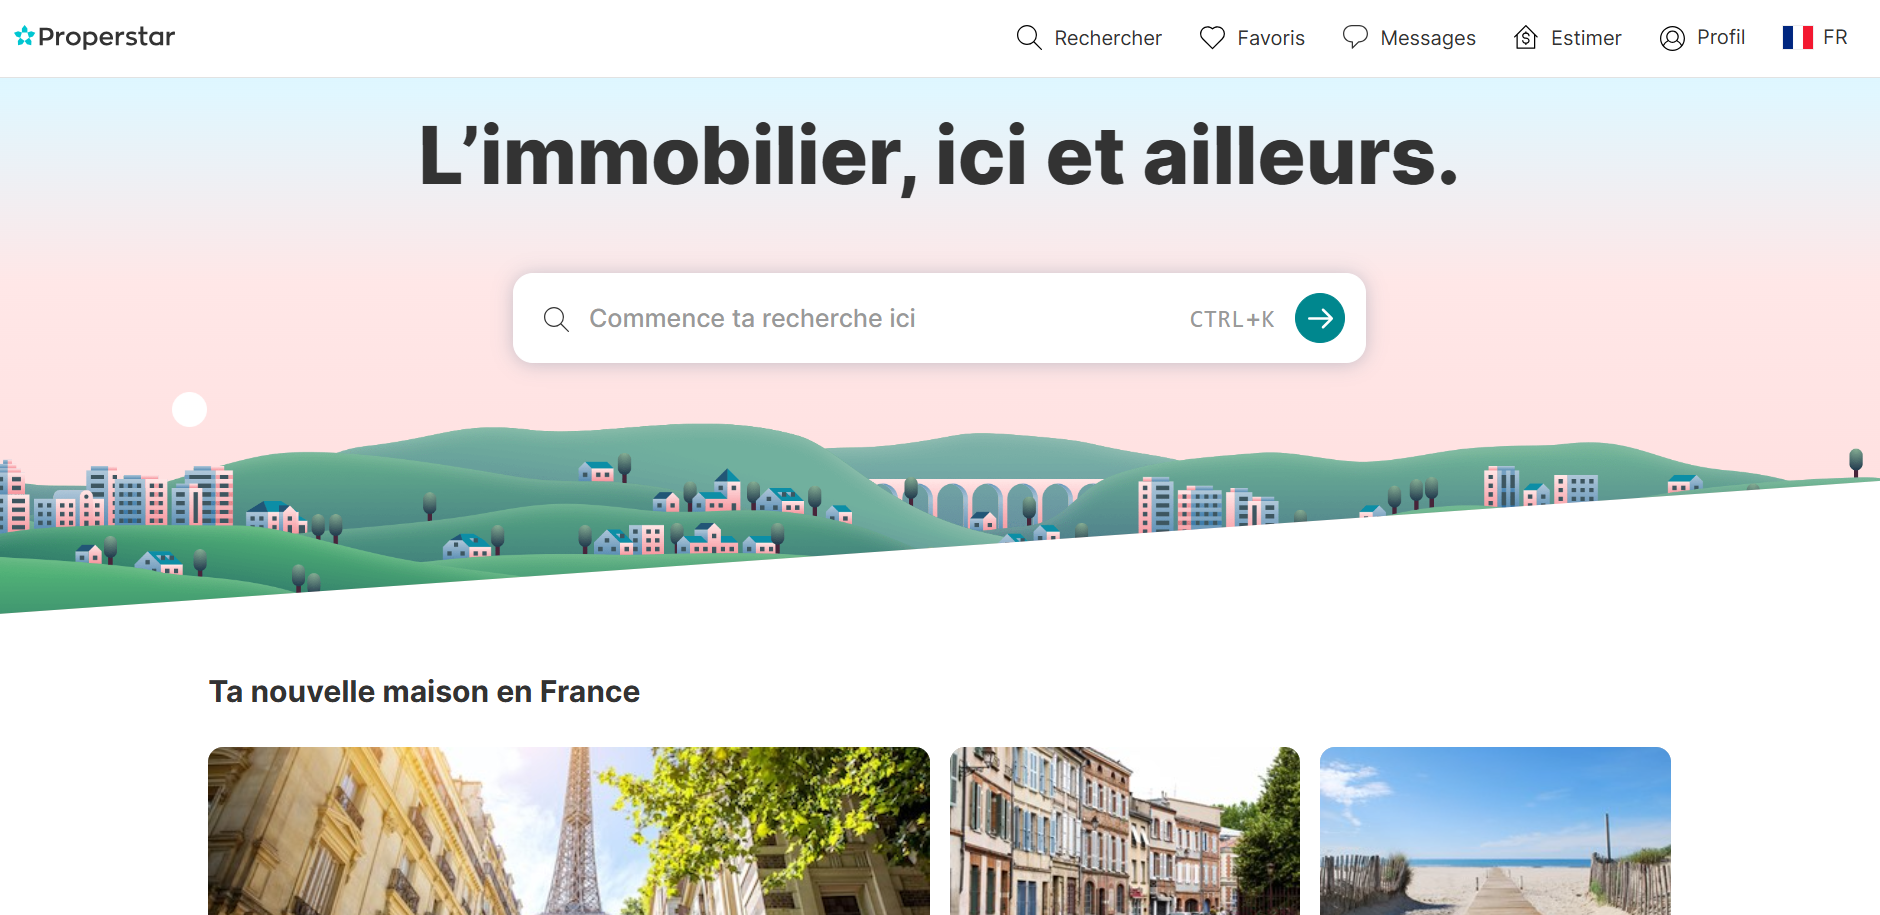
\includegraphics[width=\linewidth]{images/properstar.png}
        \caption{properstar website}
        \label{fig:properstar-website}
    \end{minipage}
    \hfill
    \begin{minipage}{0.47\textwidth}
        \centering
        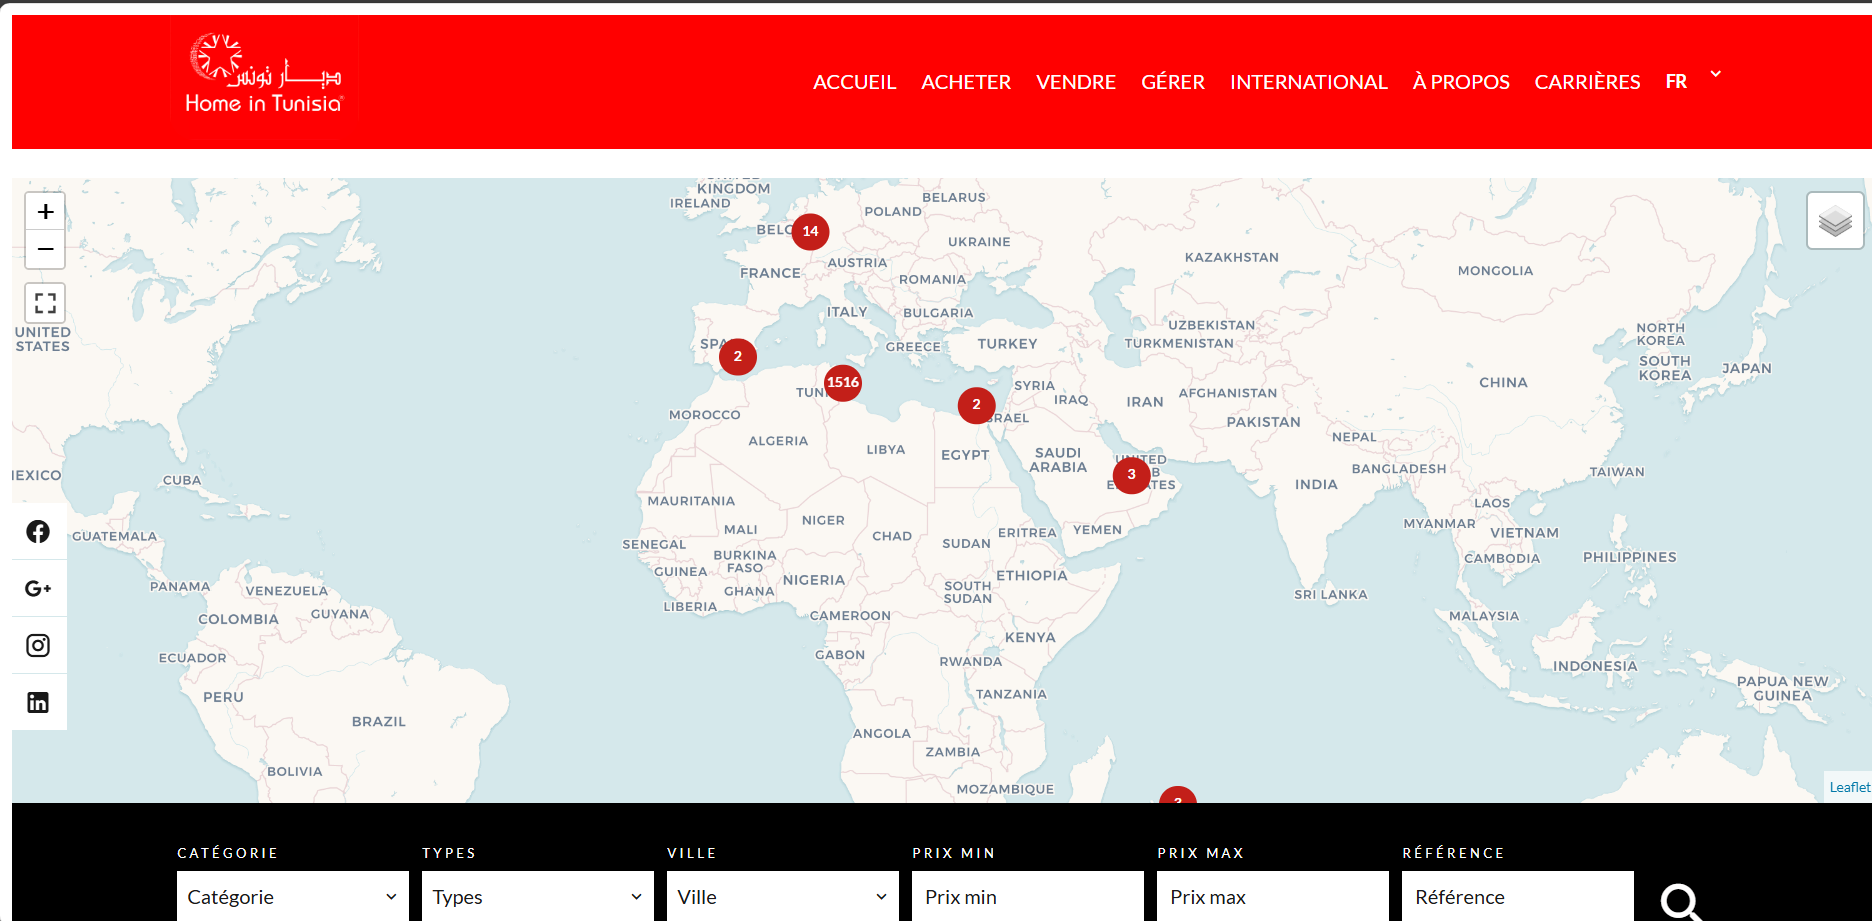
\includegraphics[width=\linewidth]{images/home_in_tunisia.png}
        \caption{homeintunisia website}
        \label{fig:homeintunisia-website}
    \end{minipage}
    
    \vspace{0.75cm}
    
    \begin{minipage}{0.47\textwidth}
        \centering
        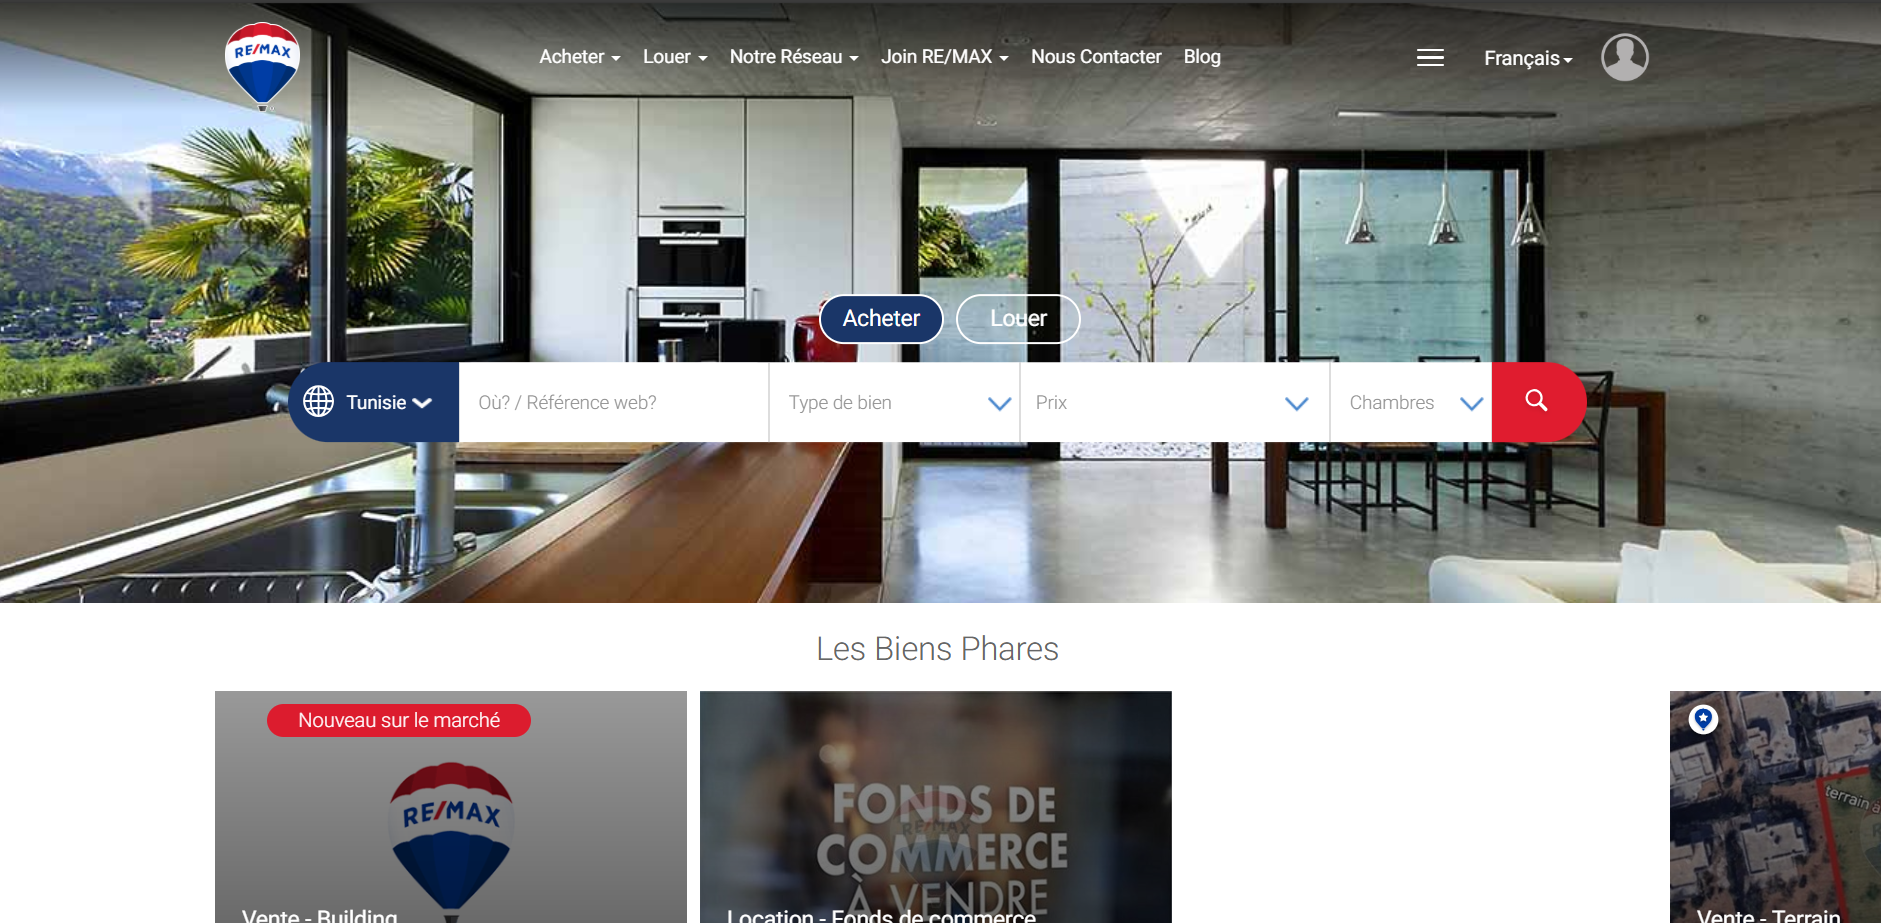
\includegraphics[width=\linewidth]{images/remax.png}
        \caption{remax website}
        \label{fig:remax-website}
    \end{minipage}
    \hfill
    \begin{minipage}{0.47\textwidth}
        \centering
        
\includegraphics[width=\linewidth]{images/mub.png}
        \caption{mubawab website}
        \label{fig:mubawab-website}
    \end{minipage}
\end{figure}


Our scraping system uses a distributed architecture with the following components:
\begin{itemize}
    \item Rate-limiting and request throttling to respect website policies
    \item Scheduled jobs for regular data updates
    \item Data validation and cleaning pipelines
\end{itemize}
\newpage
\begin{figure}[htbp]
    \centering
    % Placeholder for a diagram of the scraping workchart
    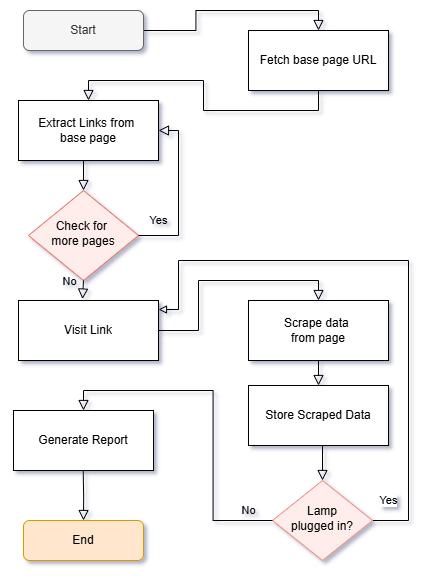
\includegraphics[width=0.55\textwidth]{images/workchartscraper.png}
    \caption{Data Scraping workchart}
    \label{fig:scraping-workchart}
\end{figure}



\section{Property Valuation Prediction Model}
\subsection{Overview}
The Property Valuation Prediction Model is designed to estimate both the market value and potential rental income for real estate properties. This provides investors with crucial information to make informed investment decisions.

\subsection{Model Architecture and Training Process}
\subsubsection{Data Features for Valuation}
The accuracy of the property valuation model heavily relies on the quality and comprehensiveness of the input data. Figure \ref{fig:geo-propriety-data} outlines the key geo-property data features utilized by the model. These features capture essential characteristics of a property and its location, enabling the model to learn complex relationships and predict market values and rental incomes effectively.

\begin{figure}[htbp]
    \centering
    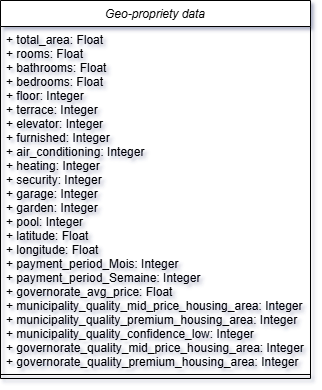
\includegraphics[width=0.4\textwidth]{images/geo-propriety-data.png} % Replace with your actual image path
    \caption{Geo-propriety Data Features for AI Models}
    \label{fig:geo-propriety-data}
\end{figure}

\subsubsection{Model Selection}
To develop an accurate property valuation prediction model, several regression algorithms were evaluated. The following models were selected for training and comparison due to their distinct characteristics and common effectiveness in similar predictive tasks:
\begin{itemize}
    \item \textbf{Linear Regression}: Chosen as a baseline model due to its simplicity and interpretability. It helps in understanding the linear relationships between the features and the target variables (market value and rental income).
    \item \textbf{Random Forest Regressor}: An ensemble learning method that operates by constructing a multitude of decision trees at training time. It is robust to overfitting, handles non-linear relationships well, and often provides high accuracy.
    \item \textbf{Gradient Boosting Regressor}: Another powerful ensemble technique that builds models in a stage-wise fashion. It is known for its high predictive accuracy and ability to optimize for various loss functions, making it suitable for complex regression tasks.
\end{itemize}
These models were trained on the prepared dataset, and their performances were evaluated to select the most suitable one for deployment in the Korpor platform.

\subsubsection{Feature Importance Analysis}
Understanding which features contribute most to the model's predictions is crucial for model interpretability and refinement. After training the selected model, a feature importance analysis was conducted. Figure \ref{fig:feature-importance} displays the top 15 most important features identified by the model. This analysis helps in validating the model's logic.

\begin{figure}[htbp]
    \centering
    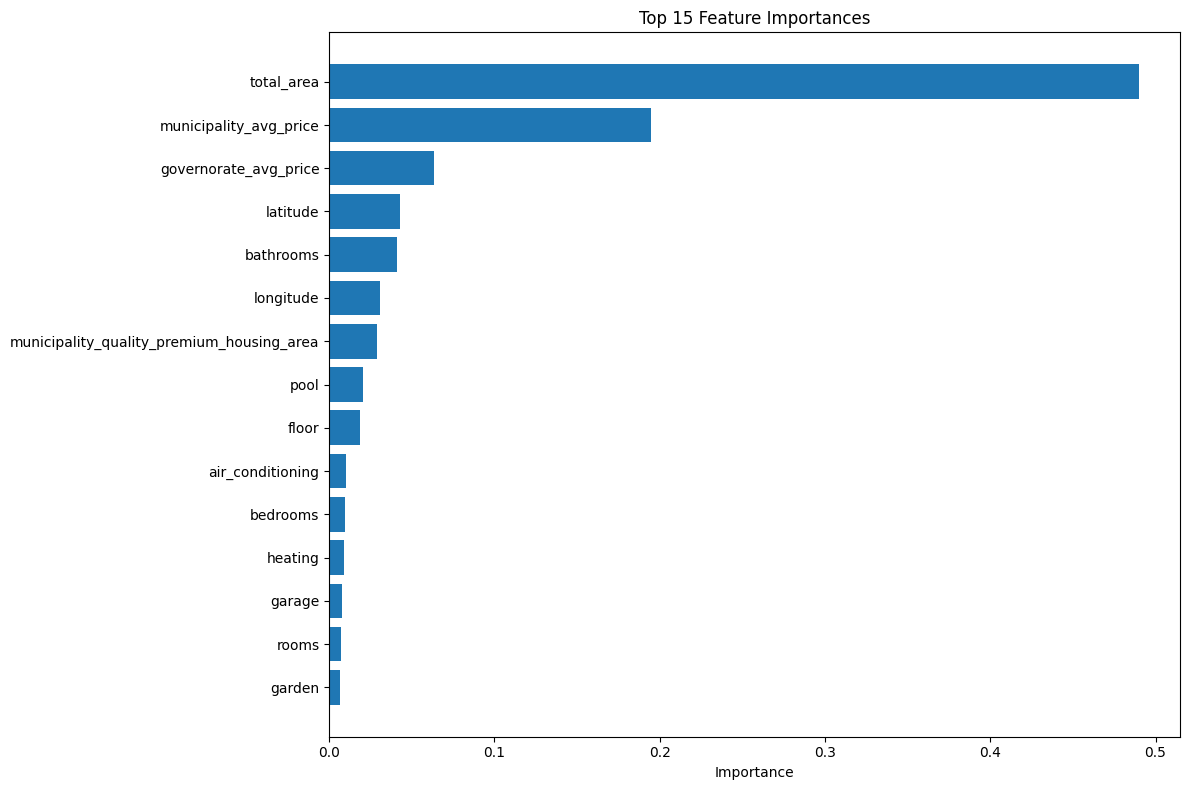
\includegraphics[width=0.8\textwidth]{images/top_15_feature_importance.png} % Assuming image is in 'images' directory
    \caption{Top 15 Feature Importance for Property Valuation Model}
    \label{fig:feature-importance}
\end{figure}

\subsubsection{Prediction Sequence Flow}
The interaction sequence for the AI property valuation prediction model is depicted in Figure \ref{fig:ai-prediction-sequence}. This diagram illustrates the flow of requests and data between the user, the application frontend, the backend server, and the AI prediction service to generate a property valuation.

\begin{figure}[htbp]
    \centering
    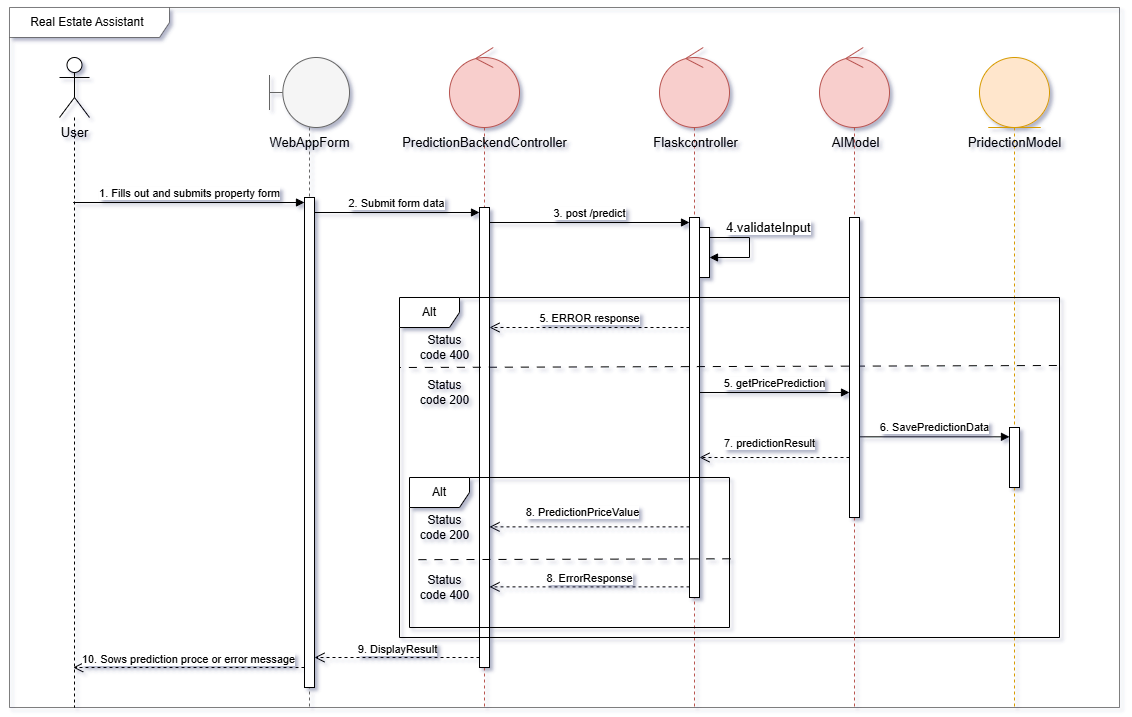
\includegraphics[width=1\textwidth]{images/sequence_AI_prediction_model.png} % Assuming image is in 'images' directory
    \caption{AI Property Valuation Prediction Sequence Diagram}
    \label{fig:ai-prediction-sequence}
\end{figure}


\subsubsection{Prediction User Interface}
The user interface for the property valuation prediction model is designed to be intuitive. Users input property details through a form, and the system displays the AI-generated valuation. Figure \ref{fig:prediction-form} shows the input form, and Figure \ref{fig:prediction-results} displays an example of the prediction results screen.

\begin{figure}[htbp]
        \centering
        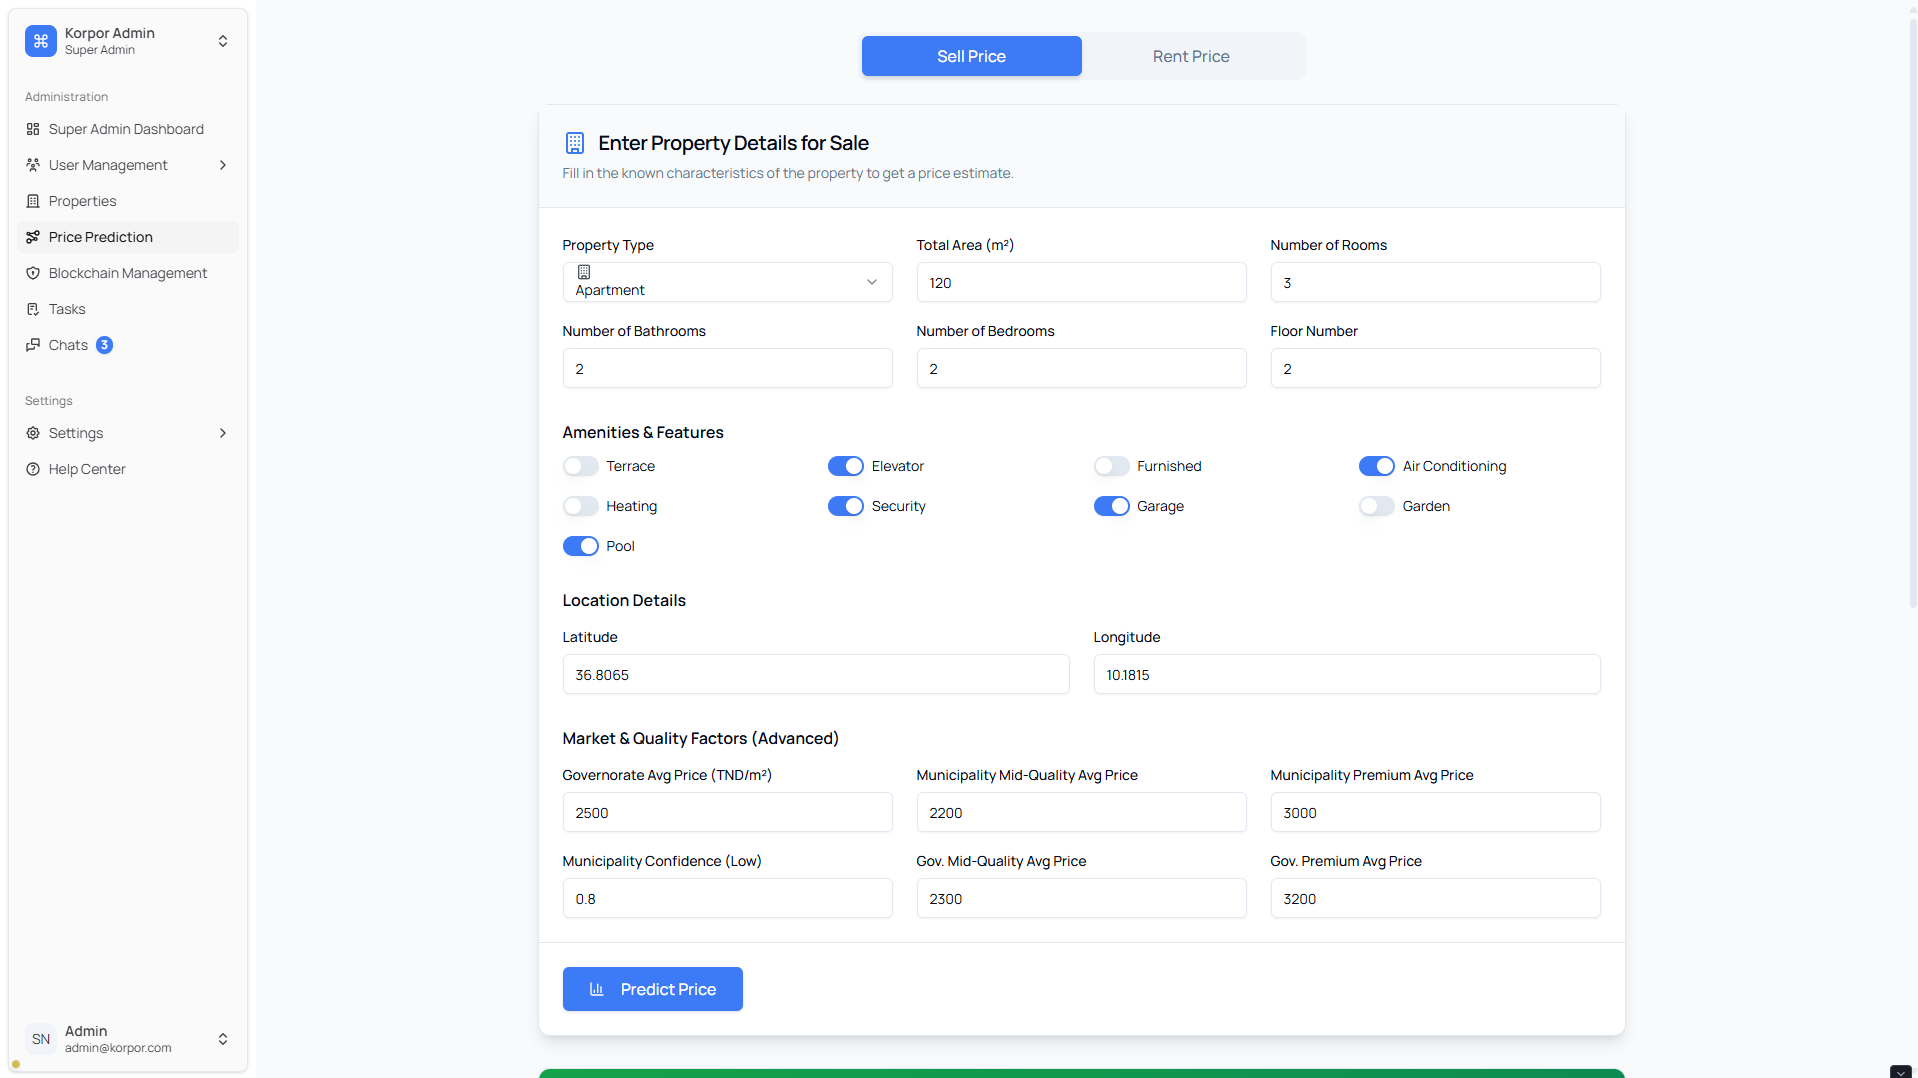
\includegraphics[width=1\textwidth]{images/screenshot_form_predition.png}
        \caption{Property Details Input Form for Valuation}
        \label{fig:prediction-form}
    \end{figure}
\begin{figure}[htbp]
        \centering
        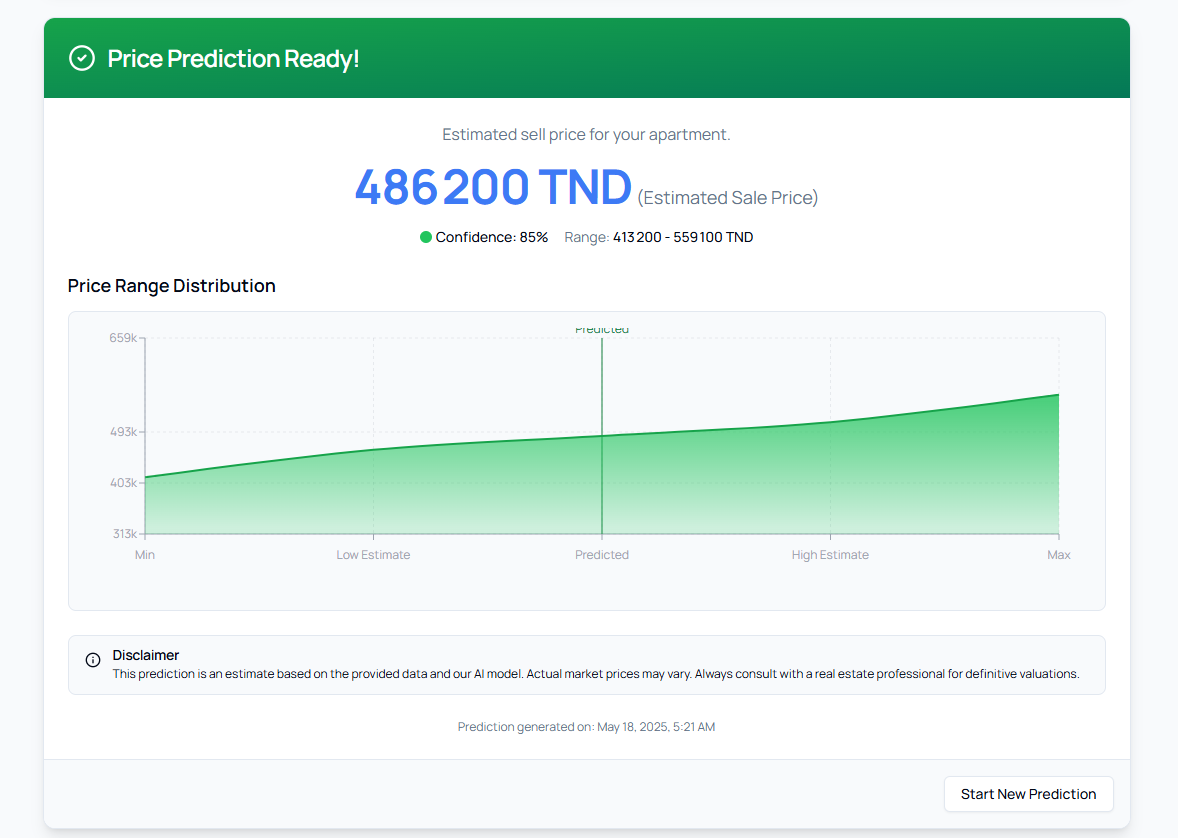
\includegraphics[width=0.7\textwidth]{images/screenshot_predctionscreen.png}
        \caption{Valuation Prediction Results Screen}
        \label{fig:prediction-results}
\end{figure}
\newpage

% \section{Real Estate Assistant}
% \section{Role-Based Backoffice Agent}
% \section{Investor-Focused Recommendation System}




